% Define document class
\documentclass[twocolumn]{aastex631}
\usepackage{showyourwork}
\usepackage{color}

\definecolor{rb4}{HTML}{27408B}
\newcommand{\kw}[1]{{\color{rb4}[KW: #1 ]}}
\newcommand{\flatiron}{\affiliation{Center for Computational Astrophysics,
Flatiron Institute, New York, NY 10010, USA}}
\newcommand{\jhu}{\affiliation{Department of Physics and Astronomy, Johns Hopkins University,
3400 N. Charles Street, Baltimore, Maryland 21218, USA}}

% Begin!
\begin{document}

% Title
\title{Turbo fast no compromise gravitational wave parameter estimation}

% Author list
\author{Kaze W. K. Wong}
\email{kwong@flatironinstitute.org}
\flatiron

\author{Maximiliano Isi}
\flatiron

\author{Thomas Edward}
\jhu

% Abstract with filler text
\begin{abstract}
We present a light-weighted, flexible and high performance framework to estimate
gravitational wave event parameters. By combining heterodyned likelihood,
automatically differentiable and accelerators compatible waveforms, normalizing
flow enhanced gradient-based MCMC, we achieve parameter estimation for real
event like GW150914 and GW170817 within a minute of sampling time with little to
no compromise. Our framework does not require pre-training or explicit
reparameterization, and can be generalized to handle higher dimensional
problems. We also discuss as near-real time parameter estimation have been shown
to be possible by multiple groups, what are the trade-offs and future
developments the community should be aware of. Our code for generating the
manuscript and running the analysis is publically available on github.
\end{abstract}

% Main body with filler text
\section{Introduction}
\label{sec:intro}

% Brief description of PE and old generation of code
Parameter estimation (PE) is one of the most commonly perform data analysis
tasks in gravitational wave (GW) data analysis. The central question of PE is to
infer the parameters of the GW source given the strain data. The PE results in
the most recent catalog of GW events are powered by a number of community
developed PE codes, including \texttt{lalinference}, \texttt{pycbc}, and
\texttt{bilby} \cite{Romero-Shaw:2020owr} \kw{cite}. These packages have been tested by a number of groups
and well regarded as the standard tools.

% Emerging tools from different group
While the standard tools have passed many robustness tests, they are known to be
computationally intensive. The exact amount of time needed to analyze one event
depends on the length of the event. These community tools take about a week to
analyze shorter events such as binary black hole (BBH) mergers, where they can
take up to a month on a computer cluster to analyze longer events such as binary
neutron star (BNS) mergers. There are efforts from multiple groups developing
tools to speed up the PE process \kw{Cite}.

%Basic idea and unique advantage of our tool

In this work, we present a light-weighted, flexible and high performance
framework to estimate GW event parameters. Our framework implemneted the
following major features to achieve its performance:
\begin{enumerate}
\item Differential waveform models
\item Normalizing flow enhanced MCMC sampler
\item Heterodyned likelihood
\item Native support for accelerator
\item JIT compilation
\end{enumerate}
\kw{Dingo can't do BNS yet}

%Structure of paper

The rest of the paper is structured as follows: We review the basic of PE in
section \ref{sec: PE}. We provide a quick summary of the sampling framework
built on top of \texttt{flowMC} in section \ref{sec: flowMC}. We present
benchmarking result in section \ref{sec: Result}. Finally, we discuss the
implications of this work and directions for future development in section
\ref{sec: Discussion}.

\section{Gravitational wave parameter estimation}
\label{sec: PE}

In this section we give a self-contained summary the gravitational-wave
parameter estimation (PE) process.

\subsection{Likelihood function}
\label{sec:likelihood}

The main objective in PE can be summarized as: given data in the form of a time
series of strain $\mathbf{d}$, find the distribution of the source parameters
$\mathbf{\theta}$ that is compatible with the data, i.e.
$p(\mathbf{\theta}|\mathbf{d})$. In order to compute this object, we can rewrite
it using Bayes' theorem,
\begin{align}
    p(\theta| d) = \frac{\mathcal{L}(d|\theta)\pi(\theta)}{p(d)},
\end{align}

where $\mathcal{L}(d|\theta)$ is the likelihood function, $\pi(\theta)$ is the
prior distribution, and $p(d)$ is the evidence. Since the evidence is a
normalization constant that does not depend on the source parameters, it is
often omitted if we are only interested in the posterior distribution. The prior
distribution is often chosen to be some simple distributions, such as uniformly
distributed in the component masses or a Gaussian distribution in the spins.
Assuming the noise follows from a stationary Gaussian process, the log
likelihood in the case of GW is given by

\begin{align}
    \log{\mathcal{L}(d|\theta)} = -\left<d-h(\mathbf{\theta})|d-h(\mathbf{\theta})\right>/2,
\label{eq: loglikelihood}
\end{align}
where $d$ is the strain data, $h(\mathbf{\theta})$ is the strain predicted by a
waveform model with a specific set of source parameters. The right handside of
eq. \ref{eq: loglikelihood} can be evaluated in either time or frequency domain.
Since it is computationally cheaper to compute the likelihood in the frequency
domain, we choose to compute the likleihood throughout this work, which can be defined as 
\begin{align}
    \left<a|b\right> = 4 Re\int \frac{a^*(f)b(f)}{\mathcal{S}_n(f)} df,
\label{eq: innerproduct}
\end{align}
where $\mathcal{S}_n(f)$ is the noise power spectral density (PSD). To compute
the integral shown in eq. \ref{eq: innerproduct}, we need to evaluate a chosen
waveform model $h(\mathbf{\theta})$ at a number of frequnecy sample points.
Evaluting the likelihood function is often the most computationally intensive
part of the PE. The most accurate waveform model is numerical relativity (NR).
However, depending on the source parameters, generating one time series of
strain using can takes a day to half a year, which makes NR prohibitably
expensive for PE. To circumvent this problem, there are a number of waveform
"approximant" families, including the IMRPhenom family \kw{}, SEOB family \kw{},
and NR surrogate family\kw{cite}. For shorter event such as a $30-30\ M_{\odot}$
BBH, one waveform call could take $10\text{ms}$ to $\sim 1s$ \kw{verify number
in lalsuite}. For longer event such as a $1.4-1.4\ M_{\odot}$ BNS event, the
evaluation time could go up to \kw{Fill}. Since one needs to evaluate the
likelihood many times during sampling\footnote{A typical PE run with
\texttt{Bilby} takes $>10^6$ likelihood evalutation to converge.}, the
computational cost in evaluating the waveform accumulate and is the main reason
of the long runtime of GW PE.

\subsection{Heterodyned likelihood}

Since the computational cost of evaluating a waveform model scales linearly with
the number of sample points either in time or frequency domain, the
computational burden for longer-duration signals are often quite large. To
reduce the computational cost, there are a number of methods to reduce the
number of basis points one would need to compute the likelihood faithfully
\kw{cite}. We use heterodyned likelihood \kw{cite} (also named relative binning
in \kw{cite}) in this work. We give a concise description of what we implement
in our code here. For more extensive discussion of the derivation of heterodyned
likelihood, we refer the reader the reference \kw{}.

\kw{Specify the idea of heterodyned likelihood here}.
The idea behind heterodyned likelihood is the following:


\begin{align}
r(f) = \frac{h(f)}{h_0(f)} = r_0(h,b) + r_1(h,b)(f- f_m(b)) + \cdots
\end{align}

\begin{align}
    \langle d|h \rangle &\approx \sum_b A_0(b) r^*_0(h,b) + A_1(b) r^*_1(h,b) \nonumber \\
    \langle h|h \rangle &\approx \sum_b B_0(b) |r_0(h,b)|^2 + 2 B_1(b) \Re[r_0(h,b)r_1(h,b)]
\end{align}


\section{\texttt{flowMC}}
\label{sec: flowMC}

In this section, we provide a high level summary of how each component in
\texttt{flowMC} benefits the sampling process and their interplay.

\subsection{MCMC with Gradient-based sampler}
\label{sec:gradient}

Given eq. \ref{eq: loglikelihood} and the prior, one can evaluate the posterior
density function over the entire parameter space of interest to obtain the most
probable set of points that are consistent with the data. However, direct
sampling quickly becomes intractable as the dimensionality of the parameter
space increases beyond a few dimensions. Markov chain Monte Carlo (MCMC) is a
common method employed to generate samples when direct sampling is not possible.

In MCMC, the posterior distribution is approximated by a Markov chain that
converges to the target distribution. The Markov chain is constructed by
iteratively proposing a new point in the parameter space based on the current
location of the chain. The proposed point is accepted with a probability that is
usually set to be proportional to the ratio of the posterior density evaluated
at the proposed point and the current point. The chain can either accept the
proposal and move to the new location, or reject the proposal and stay at the
current location. This process is repeated until the chain converges to the
target distribution. The samples generated by the chain are then used to
estimate the quantities of interest, such as the mean and credible intervals of
the source parameters. In practice, since we do not know the target distribution
ahead of time, the MCMC process is usually repeated until a certain criterion is
met, such as a Gelman-Rubin convergence statistic \cite{Gelman-rhat} lower than
a threshold or simply after a certain number of iterations.

Compared to direct sampling, MCMC algorithms only explore regions that are
highly probable, thus reducing the computational cost by not wasting resource in
region where it is unlikely to generate the data. However, MCMC algorithms come
with their own set of issue. To illustrate what difficulties a MCMC algorithms
may face, we can examine one of the most vanilla MCMC algorithm, the
Metropolis-Hastings algorithm with a Gaussian kernel. Starting at some initial
point, one can draw a proposed point from a Gaussian transition kernel, defined
as
\begin{align}
    q(\mathbf{x},\mathbf{x_0})= \mathcal{N}(\mathbf{x}|\mathbf{x_0},\mathbf{C}),
\end{align}
where $\mathbf{x_0}$ is the current location of the chain,
$\mathbf{x}$ is the proposed location, and $\mathbf{C}$ is the
covariance matrix of the Gaussian. In the simplest case, we can pick
$\mathbf{C}$ to be a diagonal matrix with a constant value, which corresponds to
an isotropic Gaussian centers around the current location with a constant variance.
And the acceptance criteria is defined as
\begin{align}
\alpha(\mathbf{x},\mathbf{x_0}) = \min\left(1,\frac{p(\mathbf{x})q(\mathbf{x_0},\mathbf{x})}{p(\mathbf{x_0})q(\mathbf{x},\mathbf{x_0})}\right).
\label{eq:Gaussian_acceptance}
\end{align}

We can see from eq. \ref{eq:Gaussian_acceptance} the acceptance rate is
proportion to fraction of volume where the posterior density at the proposed
location is higher than the current location within the Gaussian transition
kernel. If we choose the variance of the transition kernel to be too large, this
fraction will be small hence the acceptance rate will be poor. On the other
hand, if one choose the variance to be too small, nearby samples will be
correlated. In both cases, the efficiency in constructing the chain with a
target number of independent samples is suboptimal. There is often a tuning
process before we run the MCMC algorithm to find the optimal tuning parameters,
in this example the variance of the Gaussian, to ensure close to optimal
performance.

However, as we are dealing with higher dimensional problems, even the optimally
tuned Gaussian transition kernel does not guarantee good performance. In order
to have a reasonable acceptance rate, the variance of the Gaussian has to be
smaller in a higher dimensional space, which means the transition kernel is in
general making smaller and smaller step as we increase the dimensionality.

Transition kernels which leverage gradient information of the target
distribution can help to address this issue of shortening steps in a high
dimensional space. Instead of proposing a new point by drawing from a Gaussian,
one can use the gradient evaluate at the current location to propose a new
point. For example, Metropolis-adjusted Langevin algorithm (MALA) \kw{cite}
place a unit Gaussian at the tip of the gradient vector at the current position,
\begin{align}
    \mathbf{x} = \mathbf{x_0} + \tau \nabla\log{p(\mathbf{x_0})} + \sqrt{2\tau}N(0,\mathbf{I}),
\end{align}
where $\tau$ is the step size, which is a tuning parameter. Compared to a
Gaussian centers at the current location, the MALA transition kernel is more
likely to propose a point into the higher posterior density region because of
the gradient term, which helps to boost the acceptance rate.

While transition kernels that use gradient information can help to improve the
acceptance rate, computing the gradient of the posterior density function
introduce additional computational cost, which is not necessary beneficial in
terms of sampling time. If one wants to compute the gradient information through
finite differencing, the additional computation cost goes as at least $\sim
\mathcal{O}(2n)$, where $n$ is the dimension of the problem. \texttt{Jax} allows
us to compute the gradient of the likelihood function with respect to the
parameters through automatic differentiation, which gives the gradient
information down to machine precision at around the same order of time compared
to evaluating the posterior itself. Having access to gradient information
through automatic differentiation is crucial to make the trade-off between using
gradient-based transition kernels and additional computation cost favorable.



\subsection{Normalizing Flow}
\label{sec:flow}

% Problem with just HMC or MALA
While gradient-based samplers have been shown to be superior in terms of
performance when compared to other gradient-free algorithms in many practical
examples\kw{cite}, there are still a number of classes of problems
gradient-based samplers do not solve well. \footnote{To be specific, we are
referring to sampling algorithms that use first order derivative here. Sampling
algorithms that use information of higher order derivative such as manifold-MALA
and Riemannian-HMC can in principle decorrelate local correlation in the target
distribution, however they often have instability issue when they are used on
real-life application, so they are not used often in practice.} For examples,
target distribution that exhibits local correlation are hard to dealt with,
since by construction first order gradient-based algorithms can only handle
global correlation structure. Another example is multi-modality. If there are
multiple modes in the target distribution, an independent chain will likely to
be trapped in one mode and take extremely long time to transverse between the
modes. This means the relative weights between modes will much longer to sample
compared to the shape of each mode.

% Long burn-in too
Moreover, before we can use the sampling chain to estimate the quantity we care,
the sampler often needs to first find the most probable region in the target
space, which is a common process that is referred to "burn-in" in the
literature. This means one would discard a certain amount of data generated from
the beginning and only use the later part to estimate the quantities of
interest. The burn-in phase of a gradient-based sampler is often as long as the
sampling phase, which means a good portion of computation is not necessary
helpful in estimating the target quantities.

% Crux of normalizing flow
Normalizing flow is a neural-network based technique that aims at learning a
mapping between a simple distribution, such as a Gaussian distribution, to a
complex distribution, often given in the form of data samples from a target
distribution. Once the network is trained, one can evaluate the probability
density of the complex distribution and samples from it very efficiently.
The core of normalizing flow is given by
\begin{align}
    p_x(X) = p_z(Z) \left| \frac{\partial f}{\partial z}\right|,
\end{align}
where $p_x(X)$ is the complex target distribution $p_z(Z)$ is the simple latent
distribution, and $f$ is an invertible parameterized transform that
connect the two distributions. For a detail discussion of the algorithm, we
refer the readers to \kw{cite}.

% How does it help our sampling
As mentioned in the previous subsection, one of the main issue gradient-based
sampler is it does not explore local correlation and multi-modality well. This
is exactly where the normalizing flow model can help. While the method would
still work when there is only one independent local sampler chain, this method
works much better when we employ a lot of independent chains. By looking across
multiple chains, the normalizing flow learns the global landscape of the target
distribution, hence we can use it as a \textit{proposal} distribution. This
means independent chains can now jump between modes, or within a single mode
that exhibits complex geometry that cannot be handled easily only through the
local sampler, which greatly reduce both the burn-in time and sampling time.

% Write down how you use it as proposal

\begin{align}
    acc(x,x_0) = \rm{min} \left[ 1, \frac{\hat{\rho}(x_0)\rho_*(x)}{\hat{\rho}(x)\rho_*(x_0)}\right],
\end{align}
where $x = f(z), z \sim p_z(Z)$ is the proposed jump location and $x_0$ is the current position.
We can see the flow distribution is the target distribution when the accepting probability is 1.

\kw{Mention how this helps gravitational wave, gives examples.}


\subsection{Accelerators}
\label{sec:accelerators}

Modern accelerators such as GPUs and TPUs are designed to execute large scale
dense computation. They are often much more cost-efficient than using many CPUs
when it comes to solving problems that can be benefited from parallelization.
The downside of these accelerators compared to CPUs is they can only perform a
more restricted set of operation, and are often less performant when they are
dealing with problem that are serial. Parameter estimation with MCMC is a serial
problem, since each new sample generated from a chain depends on the last sample
in the chain. This means naively putting the problem on an accelerator is more
likely to harm the performance instead of improving it.


% More sample helps training normalizing flow
In this work, the use of accelerators provides two independent perks that
tremendously benefits the parameter estimation process. First, using
accelerators allow us to run many independent chains at the same time, which
benefits the training of the normalizing flow. Since we generate the data we use
to train the normalizing flow on-the-fly, the more independent data we can feed
to the training process, the higher chance the normalizing flow can learn a
reasonable representation of the global landscape of the target distribution. If
we only use a small amount of chains, we are limited to the correlated samples
from each chain, so we have to run more sequential steps to get the same amount
of independent data as compared to running more chains, where former option does
not benefit from parallelization but the latter does. In another word, being
able to use many independent chains help the normalizing flow learn the global
landscape faster in Wall time.


% GPU helps pack a shit ton of waveform evaluation
Another benefit accelerator brings is parallel evaluation of waveforms. The most
expensive part of evaluating the likelihood is generating the waveform. This is
especially significant when analysis long signals such as BNS merger, since the
cost of evaluating the waveform scales linearly with the number of time samples.
While the most accurate waveform model, numerical relativity, is a sequential
process, most of the gravitational wave models used in PE are approximants,
meaning they are fits to numerical relativity waveforms. These fitted form can
be evaluated at any given time or frequency without the need to simulate the
signals from an initial condition. This means generating a waveform from an
approximant can in fact be benefited from parallelization. Together with
heterodyned likelihood, we can evaluate the likelihood at $\mathcal{O}(10^7)$
different locations on an Nvidia A100 GPU. The high throughput of likelihood
evaluations unlocks the potential of the \texttt{flowMC} sampling algorithms.

\section{Result}
\label{sec: Result}

In this section, we provide a number of sanity checks as well as a number of real life usecases

\begin{enumerate}
    \item ppplot
    \item real-event result
\end{enumerate}

\subsection{Injection-recovery test}

To demonstrate the robustness of our pipeline, we use it to recover the
parameters of a set of simulated signals. We create a set of simulated signals
and inject them into simulated noise, generated under the Gaussian noise
assumption using the designed PSD for every detector. Then we run our pipeline
given the simulated data and determine the credible interval at the true
parameters of the injected signals. Given the set of credible value, we can
check whether the true value lies within a certain credible interval at a
reasonable frequency. If our pipeline is perfect, we should find the true
parameters lie within $x\%$ credible interval $x\%$ of the time, e.g. the true
value should lie within the $50\%$ credible interval $50\%$ of the time.
Deviation from this behavior suggests the pipeline is either over-confident or
too conservative.

% State the distribution of injected population
We sample 1000 events from the following distribution of parameters:


% Show injection pp plot
The result of the injection studies is shown in \ref{fig: ppplot}.

\begin{figure}
    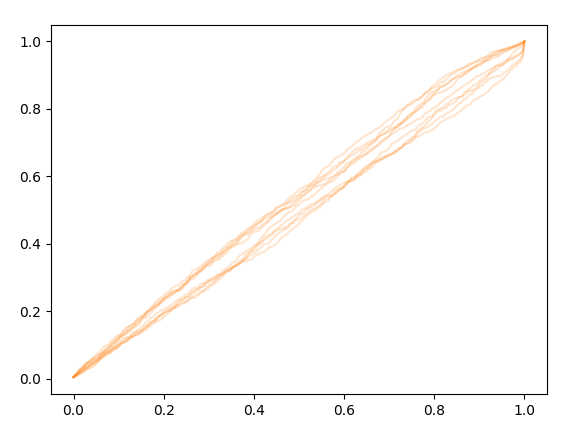
\includegraphics[width=0.99\linewidth]{static/ppplot.png}
    \caption{ \kw{I am pretty sure I am doing something wrong about the ppplot.
        Given injected q=1, there is no way the quantile is not 1, which is what
        bias the result seemingly.} }
    \label{fig:ppplot}
    \end{figure}

\subsection{Real event parameter estimation}

To demonstrate the performance of our parameter estimation pipeline, we apply
our pipeline to analysis GW150914 and GW170817. 

\kw{GW159014}

\begin{figure}
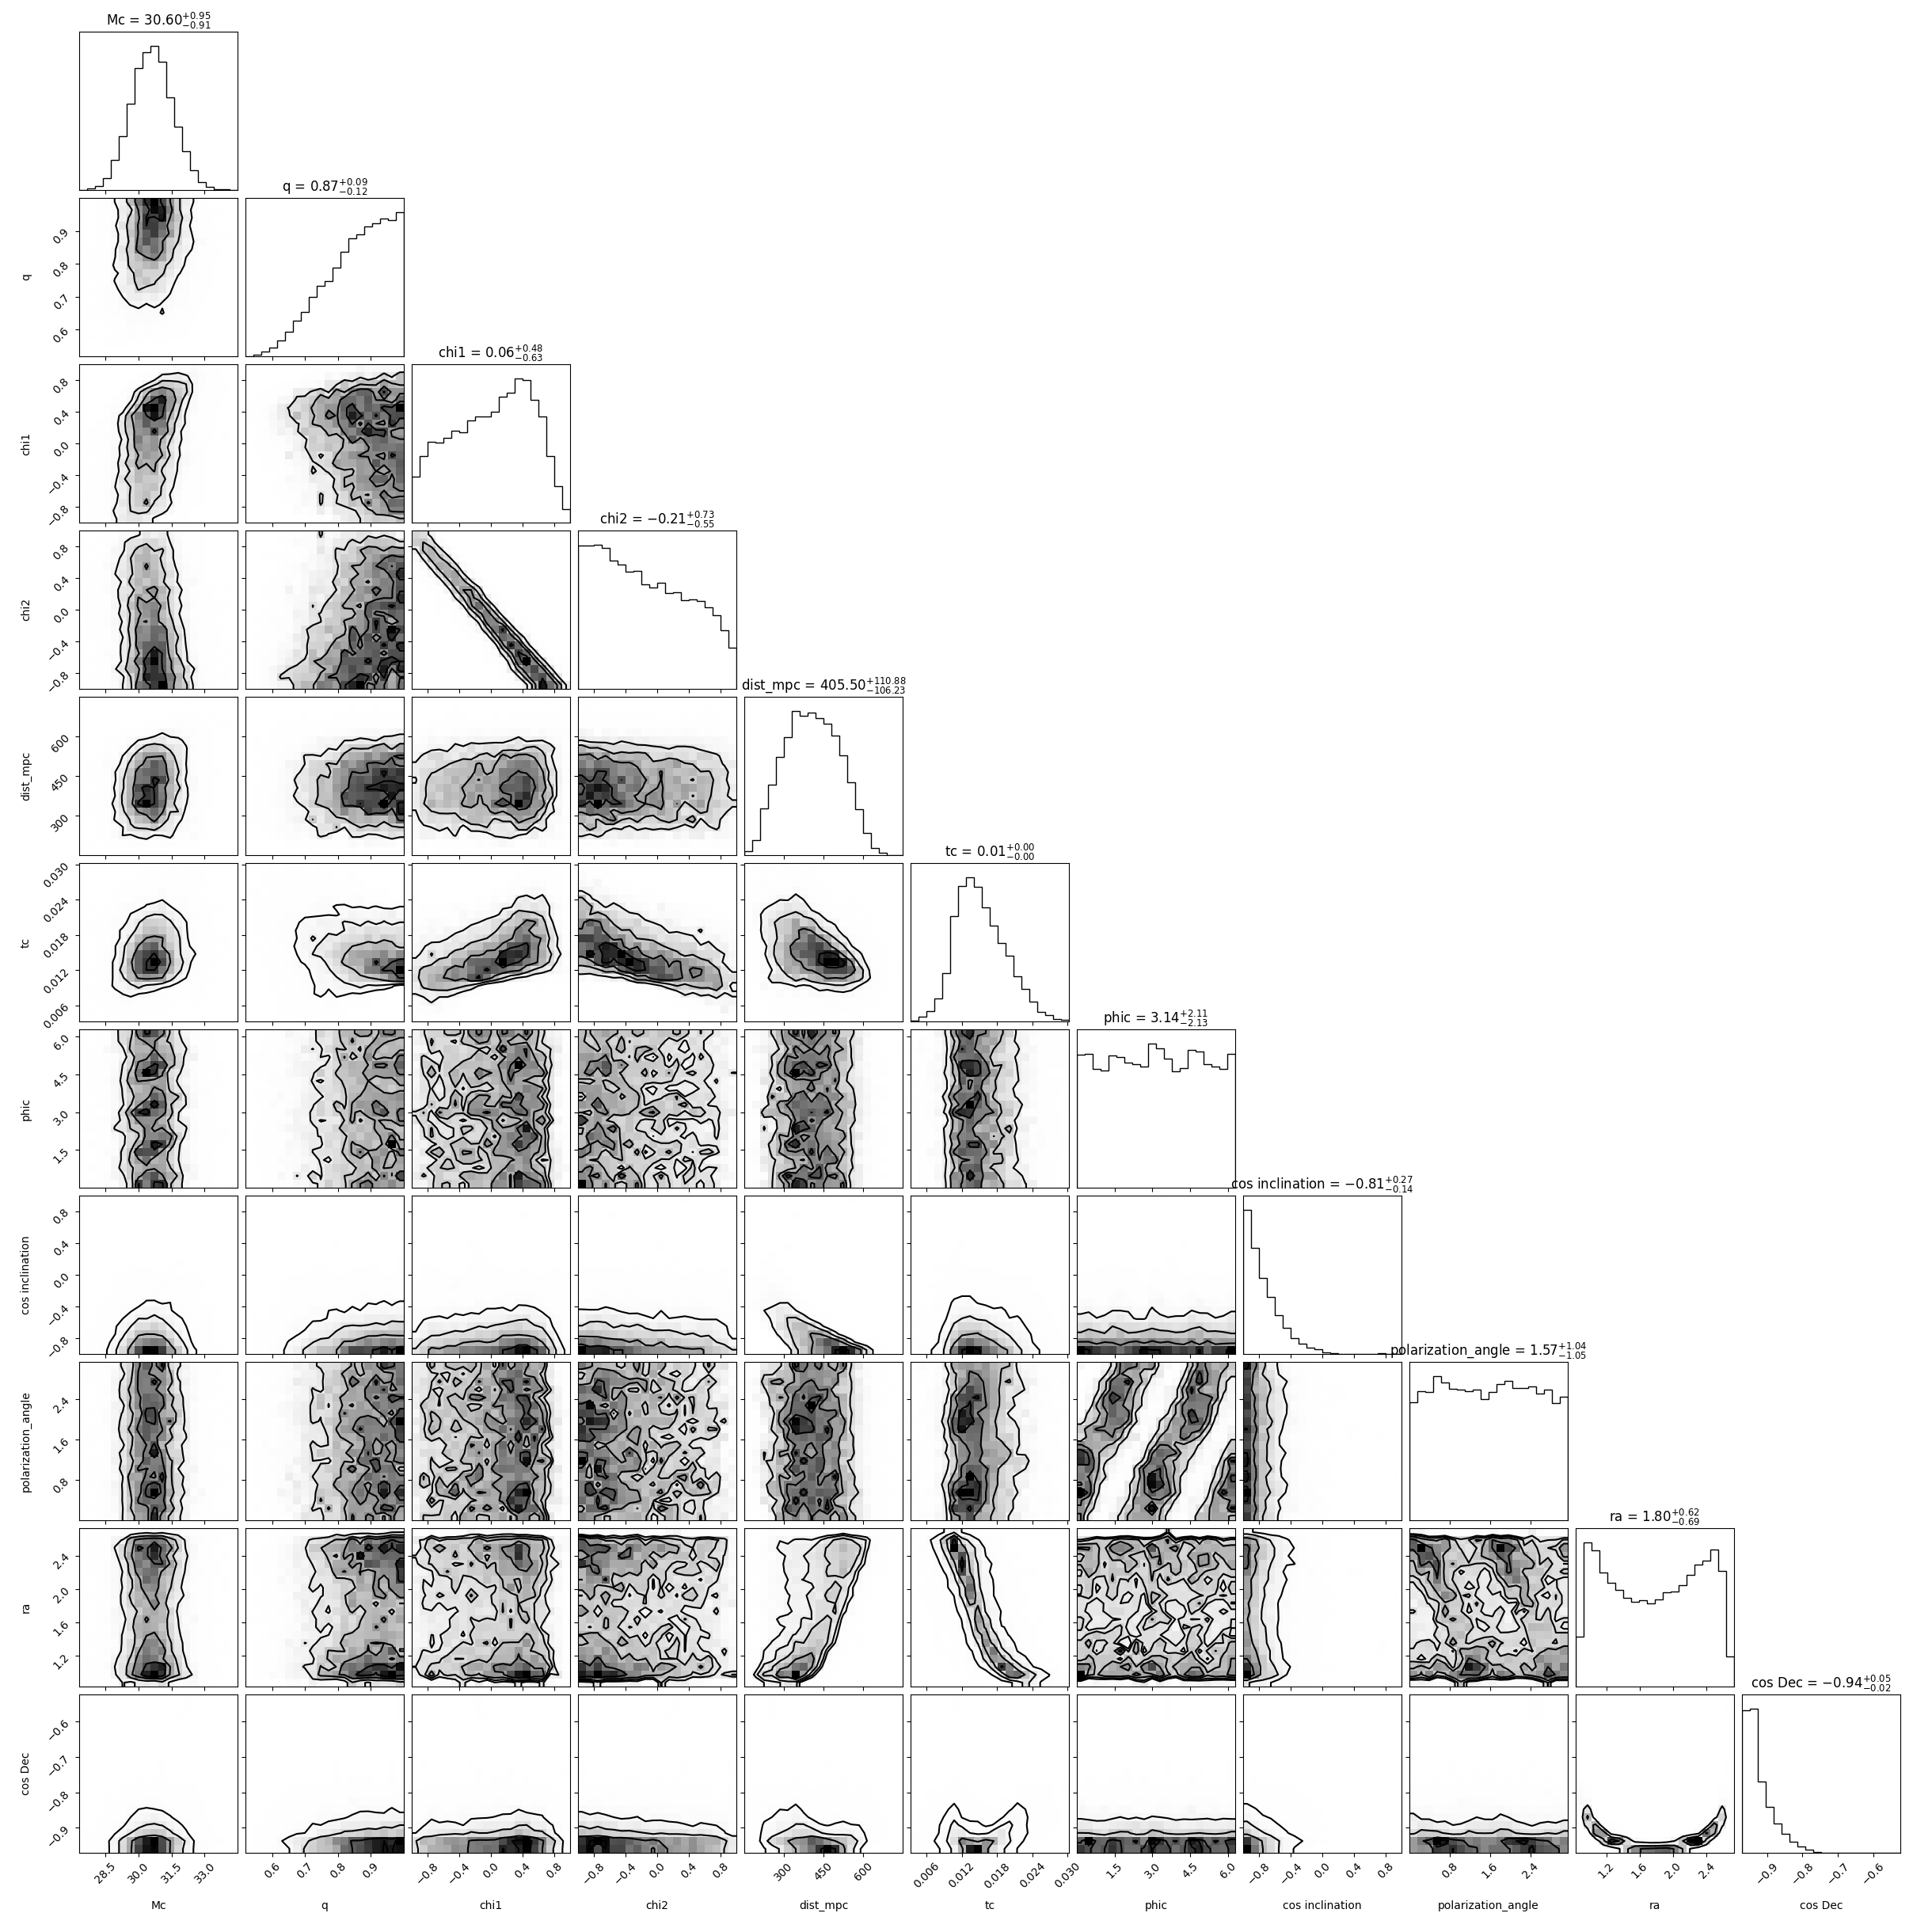
\includegraphics[width=0.99\linewidth]{static/GW150914.png}
\caption{
    hi
}
\label{fig:GW150914}
\end{figure}

\kw{GW170817}

\begin{figure}
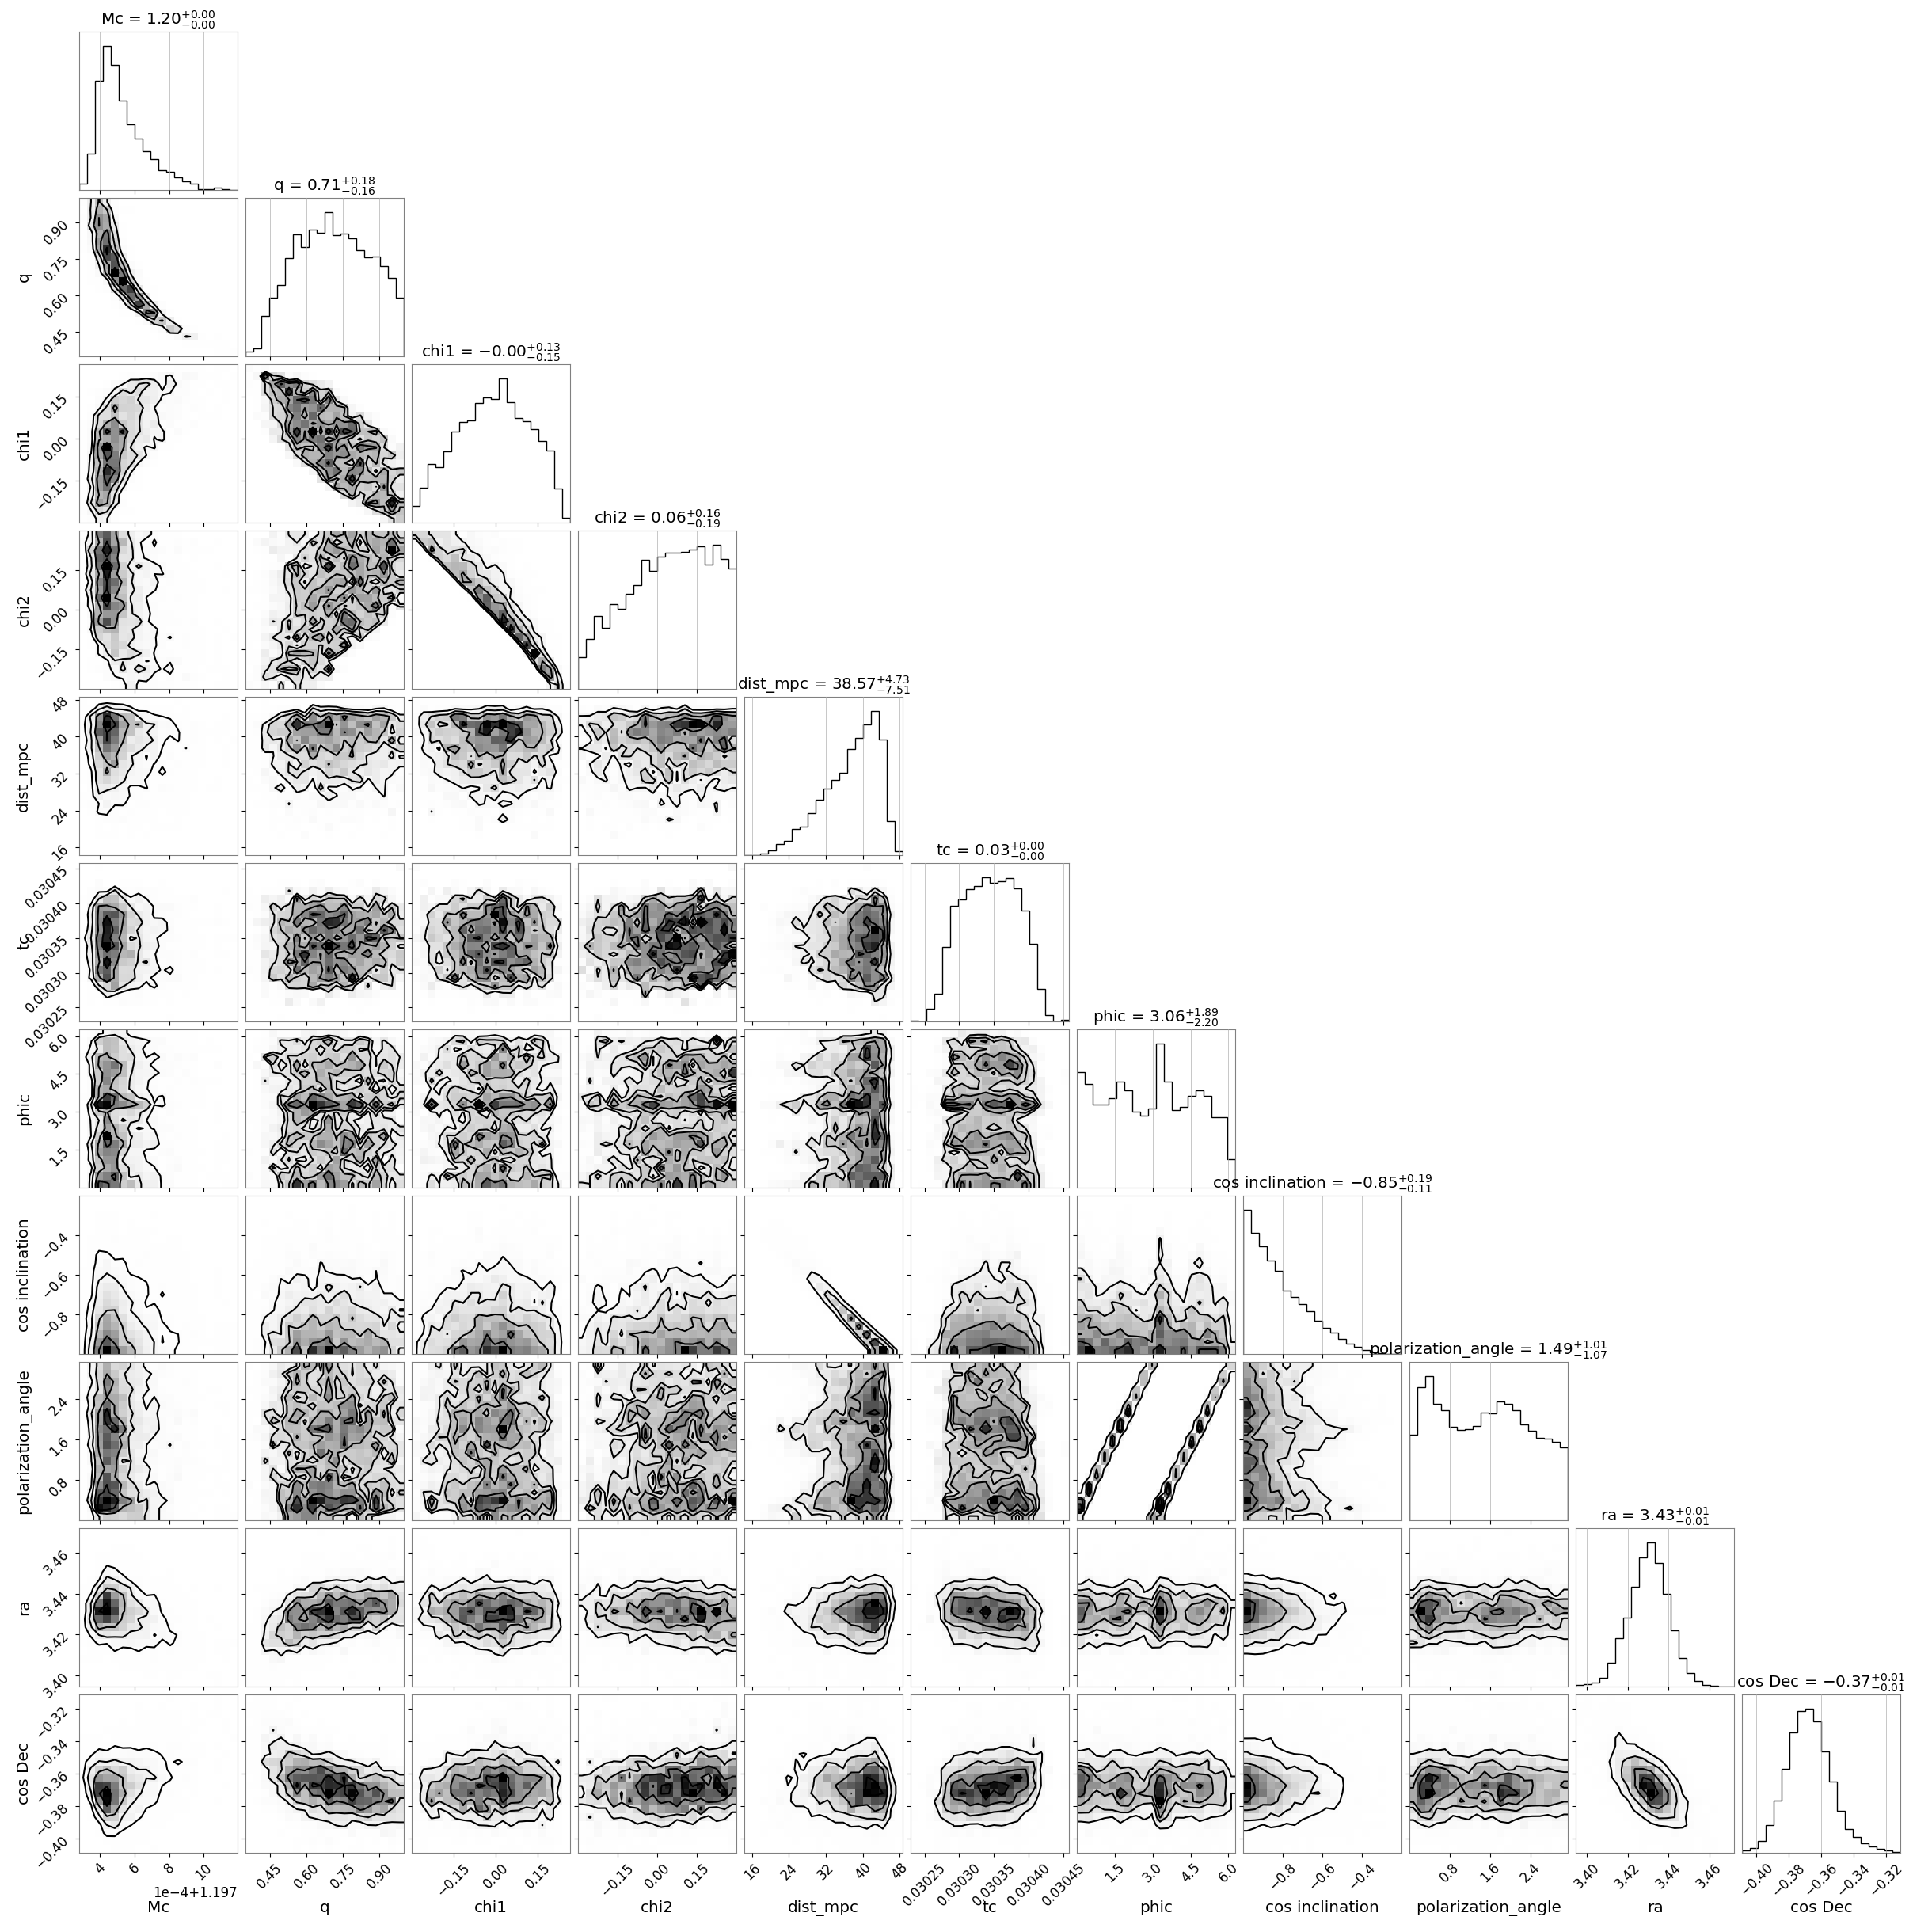
\includegraphics[width=0.99\linewidth]{static/GW170817.png}
\caption{
    hi
}
\label{fig:GW170817}
\end{figure}


\section{Discussion}
\label{sec: Discussion}

% Brief summary
In this work, we present a PE pipeline for GW events that is efficient and flexible.


% Compared to other works
There are recent works from different groups on speeding up parameter estimation
of gravitational wave, including efficient reparameterization and deep learning
\kw{cite}. While all of these methods are able to get down to minutes-scale parameter
estimation with high fidelity, we would like to highlight the unique strength of
this work, and potential interplay between our work and other's work.
% Stephen's work
Compared to \kw{Stephan's paper}, we do not rely on pre-training the
neural network on a large collection of waveforms and noise realization. This
means as soon as new waveforms models and noise models are available, our
algorithm can already be deployed. Furthermore, our met hod is essentially an
MCMC algorithm, which inherits the merit of convergence measures in MCMC. As we
are only using the normalizing flow as a proposal distribution, and the
normalizing flow is trained jointly with a local sampler, we do not suffer from
overfitting since our data is always approaching the target distribution, in
this sense, we do not introduce potential extra systematic error to inference
result.

While our pipeline use the sample generated by the local sampler for training,
one can also supply a pre-trained normalizing flow model to our pipeline to
bypass the training stage. This can further reduce the total runtime of our
inference pipeline. However, this may introduce potential systematic bias in the
inference result if the pre-trained network is not able to capture the
complexity presented in the data.

%Tousif's work
Compared to \kw{Tousif's paper}, we do not rely on handcrafted
reparameterization of the coordinate systems. If the reparameterization scheme
is known ahead of time, a nice reparameterization is also encouraged. However,
handcrafted reparameterization depends on the assumptions used in deriving the
reparameterization scheme, which would inevitably run into limitations of use
cases. Our work can be viewed as an automatic reparameterization powered by
normalizing flow, while not being exact hence as efficient as an explicit
reparameterization, the method proposed in this work is applicable to a much
boarder class of problems, such as parameter estimation with precessing
waveforms, testing GR, and multi-event joint inference.

It is always beneficial to reparameterize if the reparameterization is known
ahead-of-time. For the class of problems where \kw{Tousif's paper} is applicable
to, we can incorporate the reparameterization scheme into our MCMC pipeline to
reduce the complexity of the problem, hence speeding up the training phase.
On the other hand, if there are part of the target posterior that are not
included in the reparameterization scheme, the normalizing flow should still be
able to learn to produce accurate samples efficiently.

% Multi-modality in testing GR PE

% Access to higher dimensional problem
While standard GW analysis goes up to 17 dimensions. non-standard GW PE problems
can have more parameters, which could potentially lead to more complicate
geometry in the target posterior. For example, 

\kw{Talk about future development}


% Additional traits for having differentiable waveforms
There are a number of future developments we are working on. While IMRPhenomD is
a reasonable start, it lacks some qualitative features that other
state-of-the-art models have, such as precession and eccentricity \kw{cite}. It
also has higher mismatch with reference numerical relativity waveforms compared
to other waveforms. Currently, we are working on building differentiable
IMRPhenomX and NRSurrogate waveforms. Going forward, we encourage the waveform
development community to leverage autodiff environment such as Jax when
constructing new waveform models. Having a differentiable waveform model is not
only beneficial for parameter estimation, but also for other applications such
as calibrating waveforms to numerical relativity result, as detailed in
\kw{cite}.

% Precessing waveforms and higher mode.

% More features such as marginalization
The features we have implemented are the barebone version of parameter
estimation. We do not include marginalization schemes such as time, phase and
calibration lines marginalization. Because of the performance of the sampler on
accelerators, time and phase marginalization is not necessary, as the
performance of our implementation is not significantly impacted by having two
extra dimension. Other marginalization mode should be considered in the future.

% JIT overhead
Jax's JIT compilation drastically reduce the computational time to evaluate the
likelihood. However, it comes with a compilation overhead when the likelihood is
evaluated for the first time. We observe that the compilation time could depends
on the device where the code will be run. This is expected since Jax leverage
Accelerated Linear Algebra (XLA) to take advantage of accelerators, which means
Jax needs to compile the code for the specific device according to its
architecture. On an Nvidia A100 GPU, the compilation overhead could go up to 5
minutes for the waveform we are using. For the cases we have studied, the time
needed to obtain converging results on a A100 is about 2-3 minutes. This means
the compilation overhead is dominating the wall-clock time of the specific PE
run we considered. To utilize our implementation to its full potential, we are
looking into ways to reduce the compilation overhead, or to cache the
compilation results to avoid paying the compilation overhead for every events.

% Faster maximum likelihood finder

Another overhead we are looking into reducing is the time needed to find the
reference waveform for heterodyning the likelihood. Currently we are using
\texttt{differential evolution} available in \texttt{scipy} to find the waveform
parameters which maximize the likelihood. Since \texttt{differnetial evolution}
has not been implemented in Jax, and the Jax waveform we use is not compatible
with parallelization scheme in the \texttt{scipy} library, it takes around 5
minutes \kw{Benchmark it in the code and make this number precise.} to find the
reference waveform parameters for GW170817. There are two ways to improve the
performance in finding the parameters of the reference waveform. First, we can
explore different optimization strategy that is more compatible with the
strength of our pipeline, in particular differentiability of our likelihood and
the possibility to evaluate many waveforms in parallel with a GPU. Particle
swarm or stochastic gradient descent methods are promising candidate which we
intend to investigate in the future. 

Another way to reduce the time of finding maximum likelihood waveform is to
incoporate marginalization of extrinsic parameters to reduce the dimensionality
of the optimization problem. Currently we simutaneously maximize all 11 GW
parameters, which is unnecessarily complicated and expensive. There are
long-existing marginalization schemes over extrinsic parameters such as merger
time and phase, which can find the corresponding maximum likelihood waveform
much more efficiently when compared to differential evolution. We expect
implementing these marginalization schemes will reduce the time needed to find
the reference waveform parameters by obtaining the extrinsic parameters and by
reducing the dimensionality of the optimization problem for the intrinsic
parameters.

% Multi-device scaling

% Other detectors configuration

% Higher dimensional problems need HMC still

\section{Acknowledgements}

\bibliography{bib}

\end{document}
